\subsection{Outlier Removal}
There is a need to condition (remove stars) from data obtained from the STEREO HI spacecrafts. For this purpose the stars are treated as outlier data points from the image data obtained from STEREO. A multi step process is used to identify and remove outlier data.

STEREO HI, L2, 11 day background subtracted, DNS image data is downloaded from \url{https://www.ukssdc.ac.uk/solar/stereo/data.html}, and a first pass of star removal is preformed. This first pass consists of processing the downloaded data using the solarsoftware (SSW) IDL libraries. The stars are removed using the IDL routine \verb|subtract_star_map|, which utilizes a star map database. The data is then converted to S10 units using the SSW libraries. The result of the \verb|subtract_star_map| routine is to mainly reduce the relative brightness of stars. However, it looks as thought there is also some reduction in the number of stars. Currently the star map data base covers the data range 03/09/2007 to 01/05/2010. It is not clear as to how this effects data from 2011 on.

After applying the SSW \verb|subtract_star_map| routine, and converting the data to S10 units, the data is further processed using a MAD filter. During this process the data is split into a grid (bins). Each bin is then scanned, and a median value along with a MAD is obtained. The range of acceptable data values for the bin are determined
\begin{equation}
  \overset{\sim}{X} - k \hat{\sigma} < X_i < \overset{\sim}{X} + k \hat{\sigma}
  \label{eqn:accept_range2}
\end{equation}
Where $k$ is a parameter used to control the spread of acceptable range of data. Values that fall outside the range in \ref{eqn:accept_range2} are replaced with the $\overset{\sim}{X}$ for the bin. \textbf{Note:} One possible improvement could be to replace outliers with a local mean of data around the outlier. This method seems to remove a large portion of the stars. However, the resolution is reduced. A value of $k = 0.5$ results in the removal and replacement of about $70\%$ of the data in each bin. This requires that the bin sizes be relatively small $\left(10 \times 10\right)$ to keep a reasonable resolution.

The following images have had their brightness adjusted using ImageJ to insure a fair comparison. All images use $-32$ for the minimum displayed value, and $190$ for the maximum displayed value.
%
\begin{figure}
  \centering
  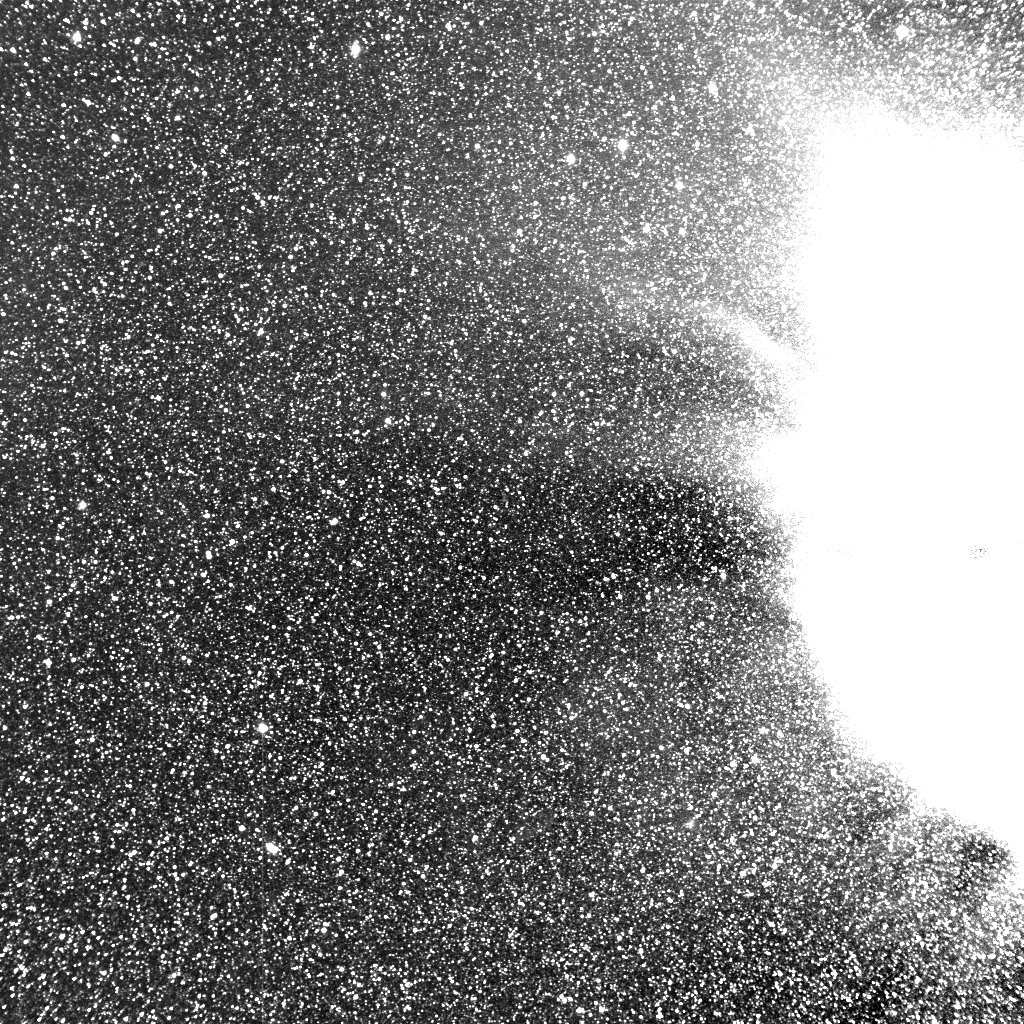
\includegraphics[scale=0.5]{../IMAGES/20110924_180901_24h1A_br11_WITH_STARS_S10_contrast_32_190.jpg} 
  \caption{STEREO HI-1A, 9/24/2011 18:09 UT, 11 day background subtraction, S10 units. Unprocessed.} 
  \label{fig:hi1a_with_stars_s10}
\end{figure}
%
\begin{figure}
  \centering
  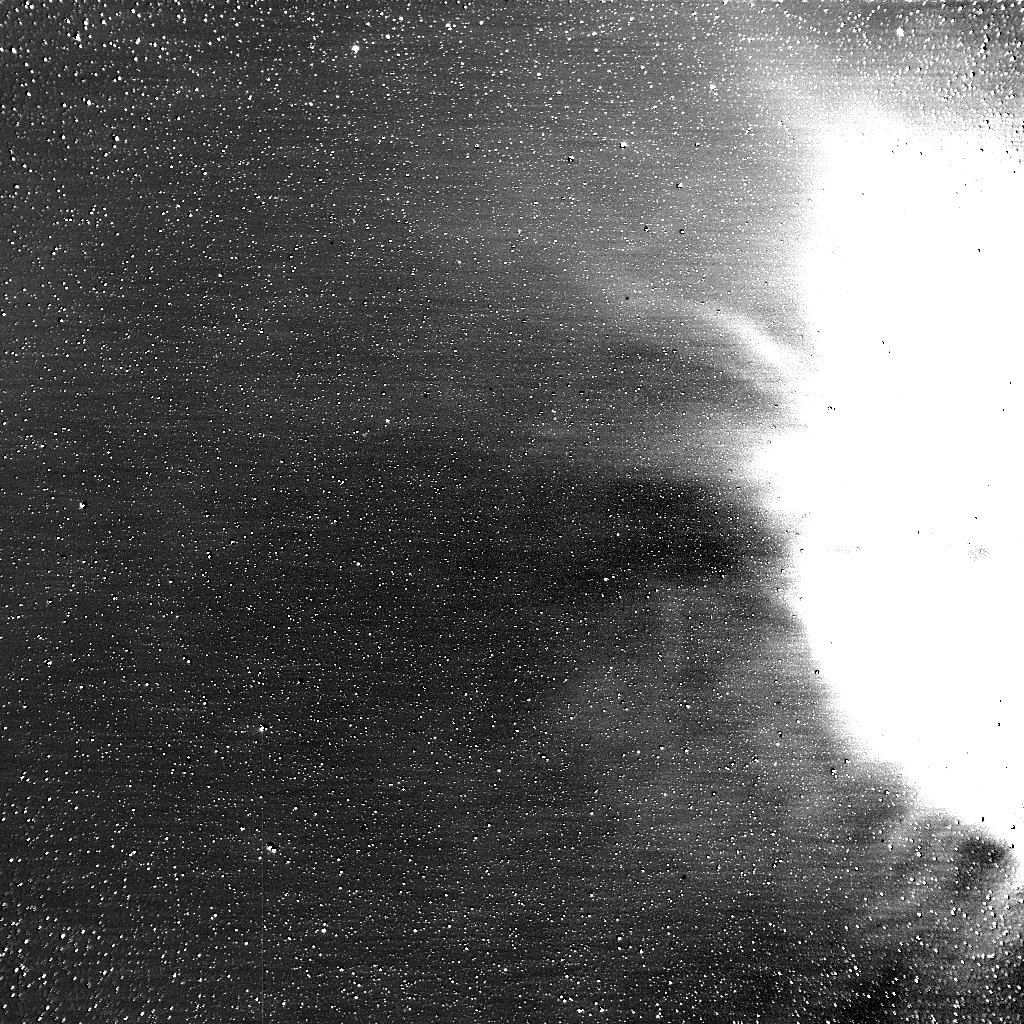
\includegraphics[scale=0.5]{../IMAGES/20110924_180901_24h1A_br11_NO_STARS_S10_contrast_32_190.jpg} 
  \caption{STEREO HI-1A, 9/24/2011, 18:09 UT, 11 day background subtraction, S10 units. Processed with subtract\_star\_map only.}
  \label{fig:hi1a_subtract_star_map}
\end{figure}
%
\begin{figure}
  \centering
  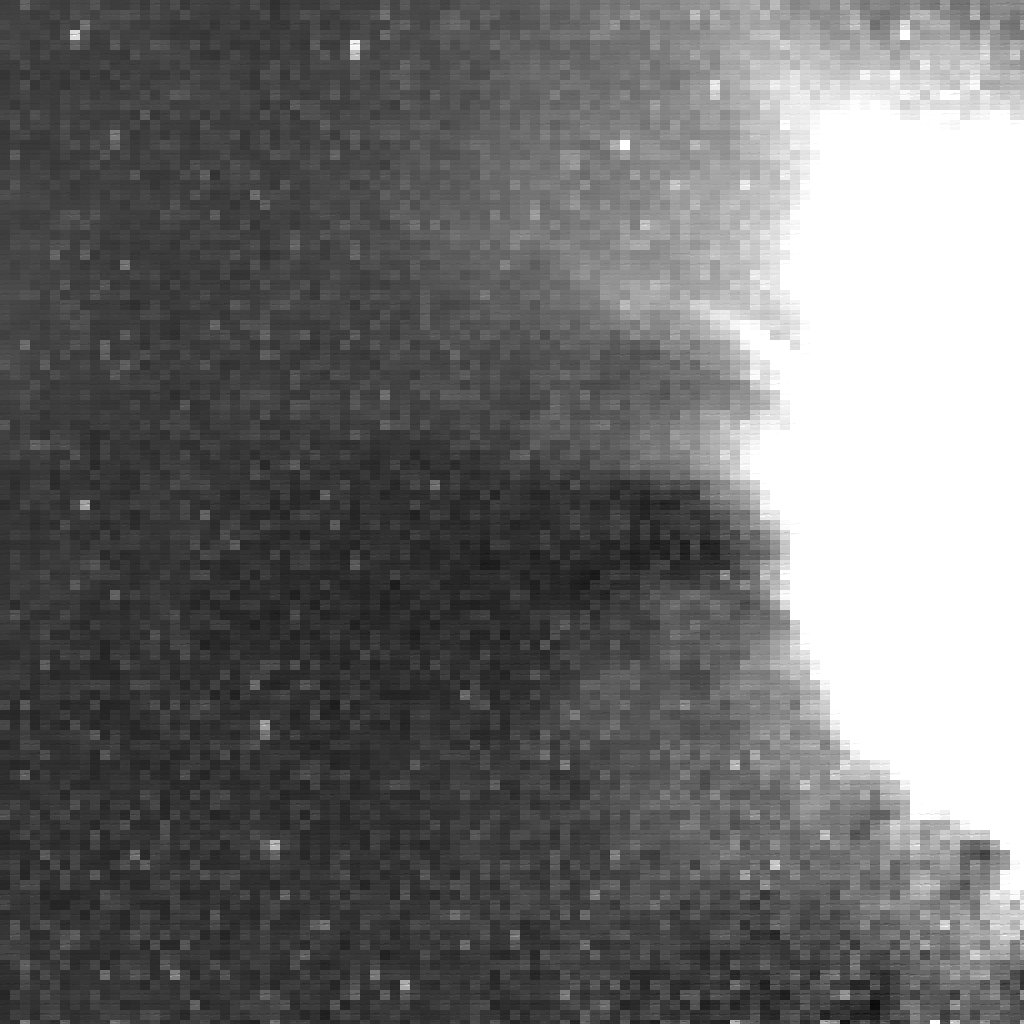
\includegraphics[scale=0.5]{../IMAGES/20110924_180901_24h1A_br11_WITH_STARS_0010_05stdev_contrast_32_190.jpg} 
  \caption{STEREO HI-1A, 9/24/2011, 18:09 UT, 11 day background subtraction, S10 units. Processed with outlier removal, with bin size $10 \times 10$, and $0.5 \hat{\sigma}$. No subtract\_star\_map routine applied.}
  \label{fig:fig:hi1a_0010bin_05stdev}
\end{figure}
%
\begin{figure}
  \centering
  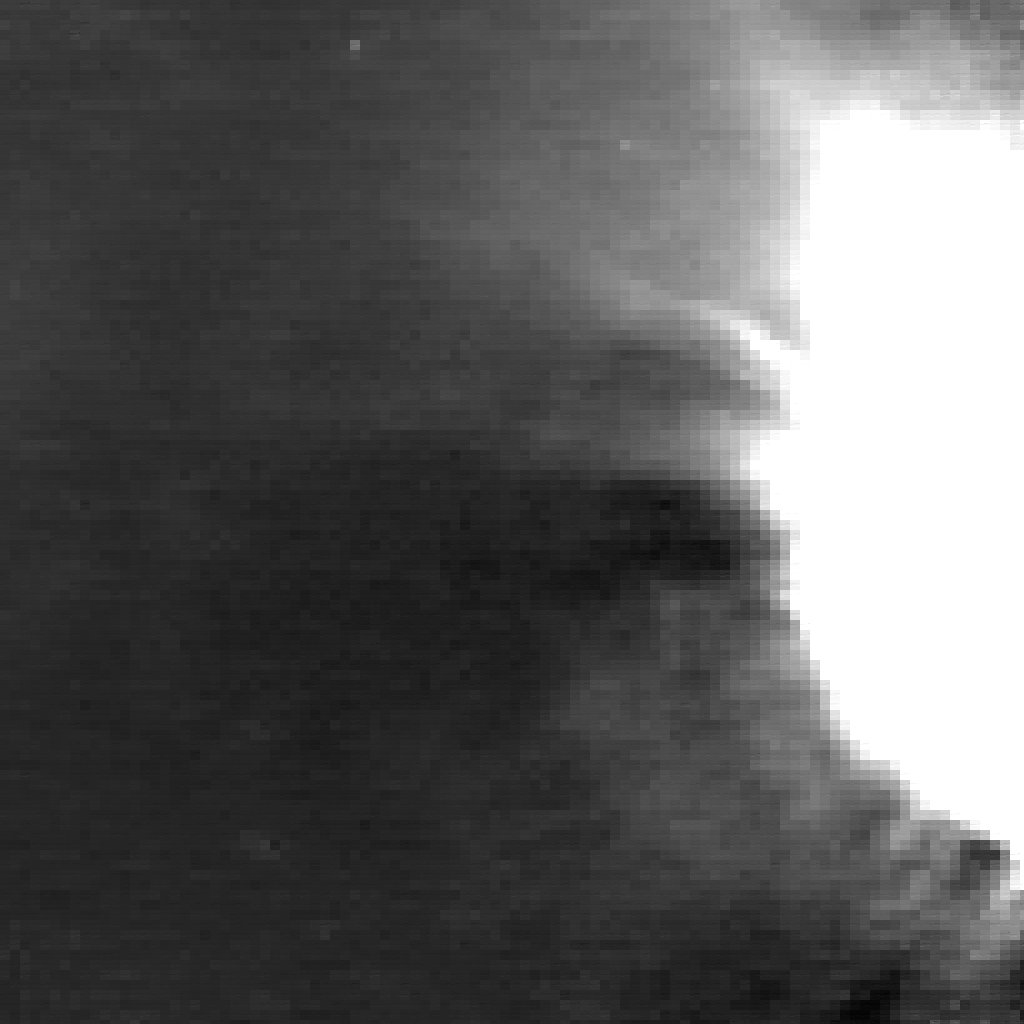
\includegraphics[scale=0.5]{../IMAGES/20110924_180901_24h1A_br11_NO_STARS_NO_STARS_0010_05stdev_contrast_32_190.jpg} 
  \caption{STEREO HI-1A, 9/24/2011, 18:09 UT, 11 day background subtraction, S10 units. Processed using subtract\_star\_map, and outlier removal with bin size $10 \times 10$, and $0.5 \hat{\sigma}$.}
  \label{fig:hi1a_subtract_star_map_0010bin_05stdev}
\end{figure}
%
























